\chapter{Basics of Terrain Rendering}
\section{Terrain Data Representation}
\subsection{Heightmaps}
One way of representing terrains is using \textit{heightmaps}.
A heightmap is a $n\times n$-grid that contains 
the height value $y$ for each $(x,z)$-position.
Positions are always spaced evenly in a grid-like manner,
but the distance between any two neighboring positions (in other words the $(x,z)$-scale) is variable.

The main advantage of heightmaps is that they allow for very simple storage and manipulation of height data, e.g. in form of images,
where low color values represent low areas of terrain and vice versa for
high color values. The color representation of an image influences the number of possible height values:
\begin{itemize}
  \item For an 8-bit grayscale image, 256 height values are supported.
  \item For a 16-bit grayscale image, 65536 height values are supported.
  \item For an 8-bit RGB image, more than 16 million height values are supported. 
\end{itemize}
Retrieving the height value for a given $(x,z)$-position is easy,
which consists of a simple lookup at the given position in the image.
Figure~\ref{fig:dom} shows a $2000 \times 2000$ heightmap of the mountain Dom in Valais, Switzerland.
\begin{figure}[H]
  \centering
  
\includegraphics[width=0.4\textwidth]{dom}
  \caption{$2000 \times 2000$ heightmap of the mountain Dom in Valais, Switzerland retrieved from SwissTopo \cite{alti3d}.}\label{fig:dom}
\end{figure}

\subsection{Triangulated Irregular Networks}
A less commonly used alternative to the heightmap is the \textit{triangulated irregular network (TIN)} data structure.
A TIN consists of a collection of 3-dimensional vertices, where 
the arrangement of vertices can be irregular. Figure~\ref{fig:tin-example} shows 
an example of a TIN.
\begin{figure}[H]
  \centering
  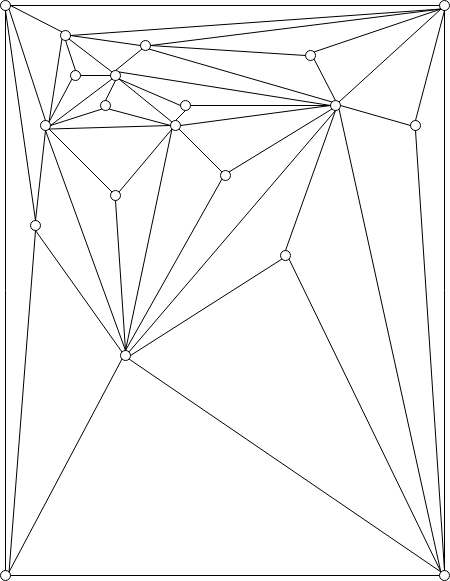
\includegraphics[width=0.52\textwidth]{tin-example}
  \caption{Example of a TIN. Note that the left area represents a terrain area with many changes 
  (e.g. mountains, hills, etc.), and the right area represents an area with few changes (e.g. flat areas).}\label{fig:tin-example}
\end{figure}

The main advantage of TINs is that fewer polygons need to be used for 
e.g. smooth terrain areas. Another advantage is that
special terrain features can be modelled 
which are usually difficult to model with heightmaps, such as overhangs, cliffs and caves \cite{lodfor3dgraphics}.
The disadvantage of TINs, however, is that the full $(x,y,z)$ coordinates need to be stored,
whereas with heightmaps, only the height value $y$ needs to be stored.
Another disadvantage of TINs is that many terrain LOD algorithms work with 
heightmaps, such as \cite{roam,geomipmapping,rottgerpaper,geomclipmaps,gpugeomclipmaps,chunkedlod,cdlod,cbt}, and not with TINs.

\section{Bintrees and Quadtrees}
\textit{Binary triangle trees (bintrees)} and \textit{quadtrees} are 
recursive data structures based on triangles and quads respectively.
Bintrees and quadtrees are mostly found in historical algorithms,
such as \cite{lindstrom1996} and \cite{roam}, but have recently been revitalized in \cite{cbt}.

A bintree consists of up to two child triangles, both of which also consist of up to two child triangles each, and so forth.
Quadtrees are structured similarly, with a quad consisting of up to four child quads, and each child quad consisting
of up to four child quads, and so forth.
Figure~\ref{fig:bintree-quadtree-example} shows an example of a bintree and a quadtree.

\begin{figure}[H]
  \centering
  \subfloat[\centering]{{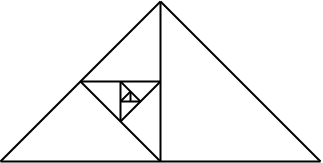
\includegraphics[width=0.43\textwidth]{bintree-example} }}
  \qquad
  \subfloat[\centering]{{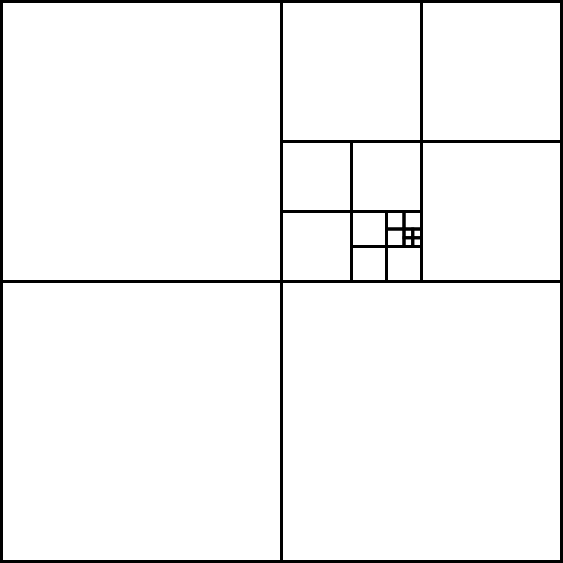
\includegraphics[width=0.33\textwidth]{quadtree-example.png} }}%
  \caption{Example of a bintree (a) and a quadtree (b).}\label{fig:bintree-quadtree-example}
\end{figure}

The main advantage of bintrees and quadtrees is that 
LOD can be modelled very naturally with them.
Bintree/quadtree sections with few children correspond to a low LOD and 
vice versa for bintree/quadtree sections with many children.

\section{View-frustum Culling}
\textit{View-frustum culling} is an optimization technique commonly used in computer graphics.
View-frustum culling is used in numerous terrain LOD approaches, such as \cite{lindstrom1996,roam,geomipmapping,geomclipmaps,cdlod}.
The \textit{view-frustum} is the 3-dimensional pyramid that represents the space that is visible to the camera.
It is defined by six planes: the near, far, left, right, top and bottom face.
Each face has a normal vector and a distance from the origin. Figure \ref{fig:view-frustum} 
shows an example of a view frustum.

\begin{figure}[H]
  \centering
  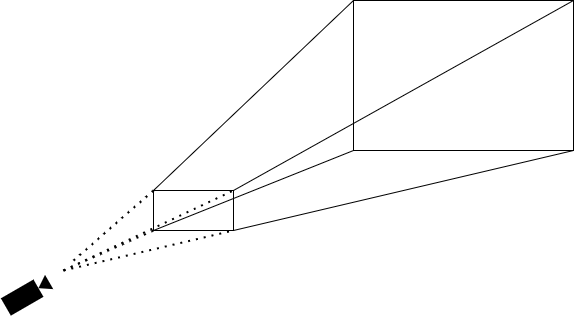
\includegraphics[width=0.62\textwidth]{view-frustum}
  \caption{Example of a view-frustum}\label{fig:view-frustum}
\end{figure}

The main idea of view-frustum culling is to check whether the \textit{bounding volume} of an object 
is contained (at least partially) inside the view-frustum, and if not, to simply not render the object.
This dramatically reduces the number of draw calls and the number of vertices that get rendered.
The bounding volume of an object is the 3-dimensional volume such that it contains the entire object inside of it.
There are different types of bounding volumes, such as \textit{axis-aligned bounding boxes (AABB)}, \textit{oriented bounding boxes (OBB)},
\textit{bounding spheres}, and more. AABB's are commonly used in terrain LOD algorithms \cite{geomipmapping,geomclipmaps,cdlod}
and are defined with two points $\mathbf{p}_{min}$ and $\mathbf{p}_{max}$, which indicate both endpoints of the AABB.
Figure \ref{fig:aabb-block} shows a terrain block with its AABB in red.

\begin{figure}[H]
  \centering
  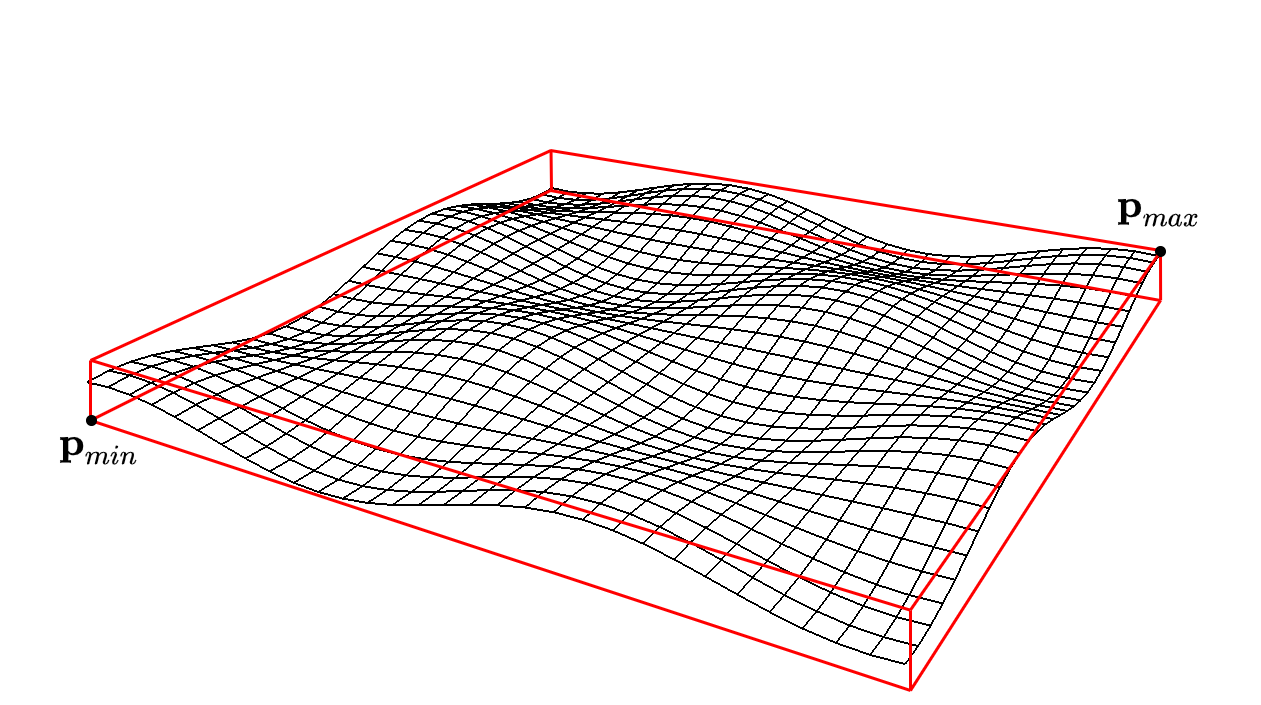
\includegraphics[width=0.72\textwidth]{aabb-block}
  \caption{Example of a terrain block with its AABB defined by $\mathbf{p}_{min}$ and $\mathbf{p}_{max}$, marked in red.}\label{fig:aabb-block}
\end{figure}

View-frustum culling can be further optimized by arranging the scene hierarchy (i.e. the terrain hierarchy)
into a \textit{space-parititioning data structure}. A widely-used structure is the already previously mentioned quadtree, where leaf nodes contain the renderable terrain sections and where
each node has an AABB that contains all bounding volumes of its child nodes.
Note that the quadtree in this case is not the same kind of quadtree from the previous section.
At render time, the quadtree gets traversed starting from the root node.
The intersection of the view-frustum with the AABB of each of the four child nodes gets calculated
and if the AABB of a child node intersects with the view-frustum, the child node gets recursively traversed
and the same steps are performed until reaching a leaf node, at which point the terrain section gets rendered.
The number of AABB-view-frustum-intersection calculations gets reduced, however at the cost of more memory consumption.
Figure \ref{fig:quadtree-frustum-culling} shows an example of quadtree-based view-frustum culling.

\begin{figure}[H]
  \centering
  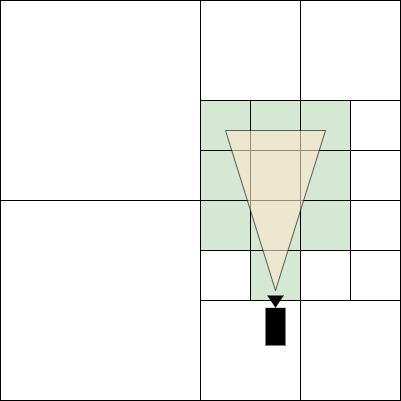
\includegraphics[width=0.4\textwidth]{quadtree-frustum-culling.png}
  \caption{Example of view-frustum culling with a quadtree viewed from the top. The view-frustum is marked in yellow and blocks that intersect the view-frustum are marked in green.}\label{fig:quadtree-frustum-culling}
\end{figure}

\section{Potential Problems During Terrain Rendering}
While terrain LOD algorithms dramatically improve the performance of terrain rendering, 
there are certain issues that can occur. 

\subsection{Cracks}
Cracks and holes in terrains can appear when a higher LOD terrain section is bordered 
by a lower LOD terrain section. The main problem is that when a vertex $v_{\text{high}}$ of a higher LOD terrain section lies on the edge $e_{\text{low}}$
of a lower LOD terrain section and the $y$ coordinate of $v_{\text{high}}$ is greater or less than the 
height of $e_{\text{low}}$ at that point, the difference in height causes the crack to appear, as shown in figure~\ref{fig:crack-example}.
\begin{figure}[H]
  \centering
  \subfloat[\centering The crack is caused by the height difference of $v_{\text{high}}$ and $e_{\text{low}}$.]{{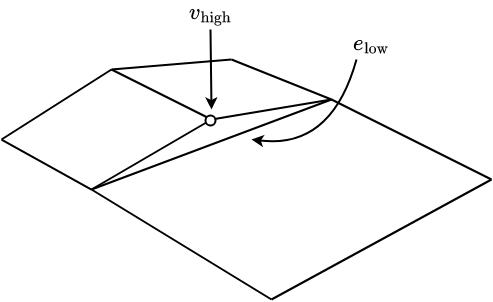
\includegraphics[width=0.5\textwidth]{crack-example} }}
  \qquad
  \subfloat[\centering The background color is set to red to highlight the cracks.]{{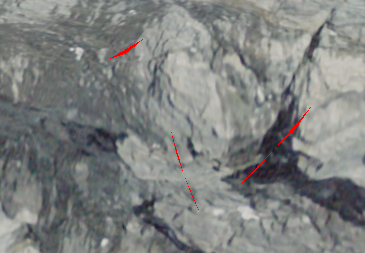
\includegraphics[width=0.4\textwidth]{cracks-terrain} }}%
  \caption{Illustration of a crack (a) and some examples of cracks in a real rendered terrain (b).}\label{fig:crack-example}
\end{figure}
Cracks can be solved by either of the following, depending on the capabilities of the LOD approach:
\begin{itemize}
  \item Removing the vertex in question, causing the higher and lower LOD meshes to be connected seamlessly (in figure~\ref{fig:crack-example} vertex $v_{\text{high}}$).
  \item Inserting an extra vertex at the border edge of the lower LOD mesh \cite[p.~194]{lodfor3dgraphics} (in figure~\ref{fig:crack-example} on top of vertex $v_{\text{high}}$). The disadvantage of this is that an extra vertex needs to get created.
  \item Covering the cracks area by rendering a strip \cite{gpugeomclipmaps}
\end{itemize}

\subsection{Popping}
The phenomenon of \textit{popping} occurs when the camera is moving 
and the transition of the terrain's LOD level causes visual pops to appear.
Popping decreases the realism of the terrain and should be as minimal as possible.
Popping can be reduced with \textit{vertex morphing} \cite{geomipmapping,geomclipmaps,cdlod}, 
i.e. by animating the transition of one LOD level to the next seamlessly through interpolation.